\section{Periodic boundaries and the crossing window}\label{sec:periodicwindow}

There are 2 ways to make Kagey's board periodic, and they are different. On a
cylinder the ball moves around a circle of pegs, and its position becomes
uniform (Remark~\ref{rem:cyl}). Here we keep the line of bins but close the
sequence of steps into a loop, so that the last step also interacts with the
first. This is the periodic Ising chain, with weight proportional to
$\exp(J\sum_{i=1}^N\sigma_i\sigma_{i+1})$, $\sigma_{N+1}=\sigma_1$ and again
$u=e^{-2J}$. Antal, Droz and R\'acz~\cite{antal2004} give its magnetization law
at a fixed scale, and Dantchev and Rudnick~\cite{dantchev2022} give exact
coefficients. We ask how much the closing bond moves the central crossing, and
then look at the row near the crossing under both boundaries.

Write $R^{\mathrm F}_{N,k}=S_{k,N-k}$ and $R^{\mathrm P}_{N,k}$ for the
bin-to-endpoint ratios under free and periodic boundaries. Put $a=k$, $b=N-k$
and $s=\sqrt{ab}$. The classical cyclic count is
\begin{equation}\label{eq:periodicratio}
R^{\mathrm P}_{N,k}(u)=\sum_{r=1}^{\min(a,b)}\frac Nr
 \binom{a-1}{r-1}\binom{b-1}{r-1}u^{2r}.
\end{equation}
To see this, note that a cyclic word with $a$ letters $\sR$ and $b$ letters
$\sL$ switches an even number $2r$ of times and has $r$ runs of each letter.
Choose compositions of $a$ and of $b$ into $r$ positive runs and a position for
the start of a distinguished run of $\sR$'s, and divide by the $r$ choices of
that run. The normalization of the periodic measure cancels in the ratio. In
particular $R^{\mathrm P}_{N,1}=Nu^2$, which gives the adjacent crossing
$J=(\log N)/4$ of Stepanyan et~al.\@~\cite{stepanyan2024}. Every interior
ratio increases strictly from $0$ to $\infty$ in $u>0$, and the ratios
increase strictly toward the middle, apart from the symmetric middle tie, by
the coefficient comparison of Proposition~\ref{prop:allbin-order}.

\begin{theorem}[periodic relative error]\label{thm:periodic-bessel}
For $N\ge2$, $1\le k\le N-1$, and $u>0$, define
\[
\widehat R^{\mathrm P}_{N,k}(u)=\frac{Nu}{\sqrt{k(N-k)}}
 I_1\!\left(2u\sqrt{k(N-k)}\right).
\]
Then
\begin{equation}\label{eq:periodicbound}
0\le1-\frac{R^{\mathrm P}_{N,k}(u)}{\widehat R^{\mathrm P}_{N,k}(u)}
\le\frac{Nu^2}{2}.
\end{equation}
\end{theorem}

In words, under periodic boundaries every bin is a single Bessel function
$I_1$, with the same kind of error as in Theorem~\ref{thm:allbin-bessel}.

\begin{proof}
Put $x=su$, $A=ab/N$, $U_r=U_r(a)$ and $V_r=U_r(b)$. Shifting the index in
\eqref{eq:periodicratio} gives
$R^{\mathrm P}_{N,k}(u)=(Nu/s)\sum_{r\ge0}U_rV_rx^{2r+1}/(r!(r+1)!)$, so the
ratio to $\widehat R^{\mathrm P}_{N,k}$ is an average of the $U_rV_r$ with
weights $x^{2r+1}/(r!(r+1)!)$, whose sum is $I_1(2x)$. By
\eqref{eq:allbin-odd-deficit}, $0\le1-U_rV_r\le r(r+1)/(2A)$, and the second
identity of Lemma~\ref{lem:clipped}(c) bounds the deficit by
$x^2/(2A)=Nu^2/2$.
\end{proof}

We can guess the next theorem. A cyclic word switches an even number of times,
so only $I_1$ appears in the periodic approximation, while the free words that
start and end on different letters give the extra $I_0$ term of the free one.
As $I_0\approx I_1$ for large arguments, the free ratio is about twice the
periodic one near the crossing. Both grow like $e^{Nu}$, so the periodic
crossing needs $Nu$ about $\log2$ larger. The same factor $2$ appears at a
fixed scale $T$ in the endpoint atoms $1/(2\cosh T)$ (periodic) and $e^{-T}/2$
(free) of Antal, Droz and R\'acz~\cite[Eqs.~(37) and~(47)]{antal2004}, while
their densities at zero magnetization agree to leading order.

\begin{theorem}[periodic crossing and boundary shift]\label{thm:periodic-crossing}
Let $u_N^{\mathrm P}$ be the positive root of $R^{\mathrm P}_{N,m_N}(u)=1$,
let $p_N^{\mathrm P}=1/(1+u_N^{\mathrm P})$, and let $u_N^{\mathrm F}=u_N$ be
the free central root. Put $c_{\mathrm P}=\tfrac12\log(\pi/2)$. As
$N\to\infty$,
\begin{align}
Nu_N^{\mathrm P}
 &=L-\tfrac12\log L+c_{\mathrm P}
 +\frac{\tfrac14\log L-\tfrac12c_{\mathrm P}+\tfrac38}{L}
 +O\!\left(\frac{(\log L)^2}{L^2}\right),\label{eq:periodicasym}\\
N(u_N^{\mathrm P}-u_N^{\mathrm F})
 &=\log2+\frac{\tfrac14-\tfrac12\log2}{\log N}
 +o(1/\log N).\label{eq:boundaryshift}
\end{align}
Replacing $Nu_N^{\mathrm P}$ by $N(1-p_N^{\mathrm P})$ preserves
\eqref{eq:periodicasym}. At the periodic crossing the coupling
$J_N^{\mathrm P}=-\frac12\log u_N^{\mathrm P}$ satisfies
\begin{equation}\label{eq:isingtemperature}
J_N^{\mathrm P}
=\tfrac12(\log N-\log\log N)
+\frac{\tfrac14\log\log N-\tfrac12c_{\mathrm P}}{\log N}
+O\!\left(\frac{(\log\log N)^2}{(\log N)^2}\right).
\end{equation}
\end{theorem}

In words, closing the loop makes every nonconstant word switch an even number
of times, so the endpoints become relatively more likely, and the periodic
chain needs about $\log2$ more expected switches before the middle catches up
with them. Since $c_{\mathrm P}=c_0+\log2$, the periodic
expansion is the free one shifted by $\log2$, with $\frac38$ in place of
$\frac18$ in the $1/L$ term.

\begin{proof}
\emph{Step 1: the first order.} At the middle $2s=N+O(1/N)$. At
$u=(1\pm\epsilon)L/N$ with fixed $\epsilon\in(0,1)$ the bound of
Theorem~\ref{thm:periodic-bessel} tends to $0$, and the large-argument form of
$I_1$ makes $\widehat R^{\mathrm P}$ tend to $\infty$ with the plus sign and
to $0$ with the minus sign. Since $R^{\mathrm P}_{N,m_N}$ increases in $u$, we
get $Nu_N^{\mathrm P}\sim L$.

\emph{Step 2: the crossing equation.} Write $z=Nu_N^{\mathrm P}$. At the root
$\log\widehat R^{\mathrm P}=O(L^2/N)$ by \eqref{eq:periodicbound}. Replacing
the argument $2su$ by $z$ changes it by $O(L/N^2)$, and
$I_1(z)=e^z(2\pi z)^{-1/2}(1-3/(8z)+O(z^{-2}))$~\cite[Eq.~10.40.1]{dlmf}. So
\[
z+\tfrac12\log z=L+c_{\mathrm P}+\frac3{8z}+O(z^{-2}+L^2/N),
\]
and Lemma~\ref{lem:inversion} with $\ell=L$, $C=c_{\mathrm P}$ and
$B=\frac38$ gives \eqref{eq:periodicasym}. As $N(u-u/(1+u))=O(L^2/N)$ for
$Nu=O(L)$, it also holds for $N(1-p_N^{\mathrm P})$.

\emph{Step 3: the shift and the coupling.} By \eqref{eq:zN},
$Nu_N=z_N+O(L^2/N)$. Subtracting \eqref{eq:thirdorder}, where
$c_0=c_{\mathrm P}-\log2$ and the correction is $\frac18$, gives
\eqref{eq:boundaryshift}, even with error $O((\log L)^2/L^2)$. Finally
$J=-\frac12\log u=\frac12(L-\log z)$, and
$\log z=\log L-(\frac12\log L-c_{\mathrm P})/L+O((\log L)^2/L^2)$ gives
\eqref{eq:isingtemperature}.
\end{proof}

Stepanyan et~al.\@~\cite[Eq.~(16)]{stepanyan2024} approximate the periodic
crossing by $\beta J\approx(2\log N-1)/5$, and their Fig.~1(b) fits the line
$\beta J\approx0.3864\log N-0.21055$. At $N=10^5$ the exact periodic crossing
is $J=4.576$ (their $\beta J$). Their Eq.~(16) gives $4.405$, their line gives
$4.238$, and \eqref{eq:isingtemperature} without its error term gives $4.578$.
The line is accurate for $10\le N\le100$ (at $N=100$ it gives $1.569$ and the
exact value is $1.574$), but it has no $\log\log N$ term.

Now we look at the whole row near the crossing. How many bins are above the
endpoints just past the crossing, and how does their height fall off away from
the middle? The factor $e^{-2y^2}$ in the next theorem is easy to guess.
Moving $yN/\sqrt{\log N}$ away from the middle multiplies the Bessel argument
by $2\sqrt{k(N-k)}/N\approx1-2y^2/\log N$. The argument is about $\log N$, so
it drops by about $2y^2$, and the ratio, which grows like $e$ to the argument,
drops by about the factor $e^{-2y^2}$.

\begin{theorem}[spatial crossing window]\label{thm:critical-window}
Let $X\in\{\mathrm F,\mathrm P\}$ and let $u_N^X$ be its exact central
crossing. For fixed real $t,y$ set
\[
u=u_N^X+\frac tN,\qquad
k_N(y)=\operatorname{nint}\!\left(\frac N2+\frac{yN}{\sqrt{\log N}}\right),
\]
where either nearest-integer convention may be used. Then, as $N\to\infty$,
uniformly on compact sets of $(t,y)$,
\begin{equation}\label{eq:criticalprofile}
R^X_{N,k_N(y)}(u_N^X+t/N)\longrightarrow e^{t-2y^2}.
\end{equation}
If $M_N^X(t)$ is the number of interior bins with probability strictly above
the endpoint probability at that parameter, then
\begin{equation}\label{eq:criticalcount}
\frac{\sqrt{\log N}}N M_N^X(t)\longrightarrow\sqrt{2\max(t,0)}.
\end{equation}
\end{theorem}

In words, the crossing window has width about $1/N$ in $u$ and about
$N/\sqrt{\log N}$ in space, and inside it the row is a Gaussian bump times
$e^t$. A weak limit theorem cannot give this, since it says nothing about a
single bin such as the endpoint.

\begin{proof}
\emph{Step 1: the profile.} Put $\delta=k/N-\frac12$ and
$\eta=2\sqrt{k(N-k)}/N=\sqrt{1-4\delta^2}$. For the stated rounding and
bounded $y$,
\[
\eta=1-\frac{2y^2}{L}+O\Bigl(L^{-2}+\frac1{N\sqrt L}\Bigr),
\qquad Nu_N^X=L+O(\log L).
\]
So the Bessel argument $Nu\eta$ at $(u,k)$ is $Nu_N^X+t-2y^2+o(1)$, uniformly
on the compact set. By Theorems~\ref{thm:allbin-bessel}
and~\ref{thm:periodic-bessel} both ratios are within relative error
$O(L^2/N)$ of their Bessel forms, and $I_0(z)$ and $I_1(z)$ equal
$e^z(2\pi z)^{-1/2}(1+O(1/z))$~\cite[Eq.~10.40.1]{dlmf}, so the prefactors
relative to their central values tend to $1$ uniformly. The change of argument
gives $e^{t-2y^2}$, and the exact central ratio is $1$, which proves
\eqref{eq:criticalprofile}.

\emph{Step 2: the count.} The interior ratios increase toward the middle. If
$t\le0$, the central ratio is at most $1$, so no interior bin is above the
endpoint. Let $t>0$ and $0<\epsilon<\sqrt{t/2}$. By Step~1, for large $N$ the
bins at scaled distance less than $\sqrt{t/2}-\epsilon$ are above the endpoint
and those at distance $\sqrt{t/2}+\epsilon$ are below, and by monotonicity so
are all farther bins. Count the bins in between, divide by $N/\sqrt L$ and let
$\epsilon\downarrow0$. Rounding changes the count by $O(1)$.
\end{proof}

Figure~\ref{fig:window} shows the exact ratios at $N=10^6$.

\begin{figure}[t]
\centering
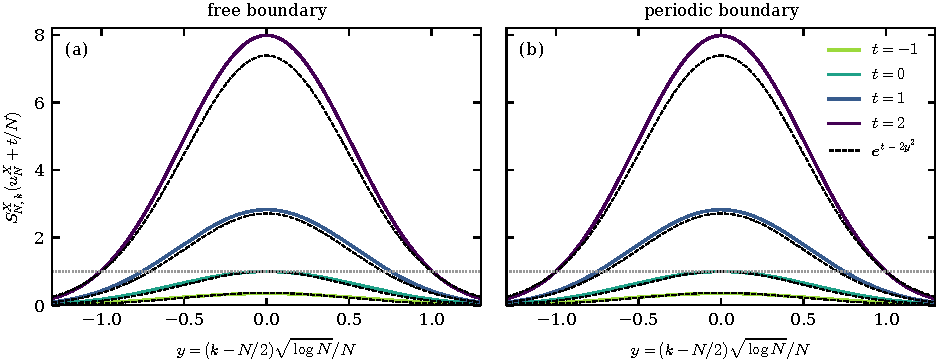
\includegraphics{figures/window}
\caption{The exact ratios $R^X_{N,k}(u_N^X+t/N)$ at $N=10^6$ for free (a) and
periodic (b) boundaries, with the limit $e^{t-2y^2}$ of
Theorem~\ref{thm:critical-window} (dashed). Here $y=(k-N/2)\sqrt{\log N}/N$,
and the bins above the dotted line are above the endpoint height. The
convergence is slow, and at $t=2$ and $y=0$ the relative error is still $0.08$.}
\label{fig:window}
\end{figure}
